\section{Durchführung}
\label{sec:Durchführung}

Für diesen Versuch wird eine Schaltung verwendet wie sie in \autoref{fig:schaltung} zu sehen ist.
Die Probe wird zwischen die Polschuhe eines Permanentmagneten gesteckt und um die Probe liegt eine Probenspule, die mit der Schaltung verbunden ist.

Zur Molekülradius Berechnung und zum Vergleich von Literaturwerten wird vor dem Versuch und nach dem Versuch die Temperatur zwischen den Polschuhen gemessen.

\begin{figure}
    \centering
    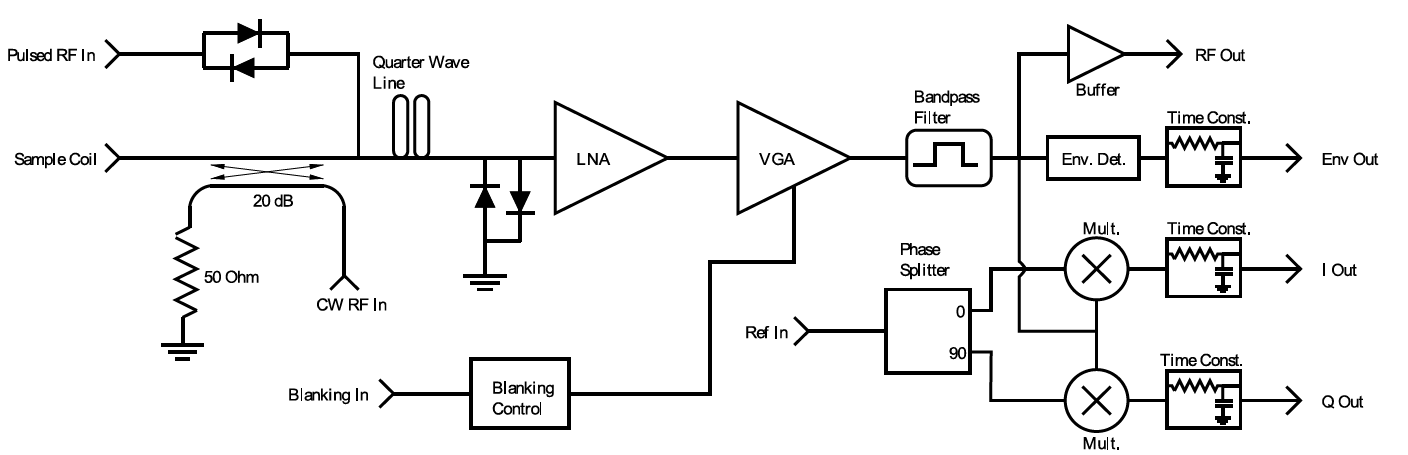
\includegraphics[width=\textwidth]{images/schaltung.png}
    \caption{Für den Versuch verwendete Schaltung \cite{teachspin}}
    \label{fig:schaltung}
\end{figure}

Am Gerät ist es möglich eine Pulsfolge wie in \autoref{fig:pulsfolge} angedeutet einzustellen und die Induktionsströme der FID auf einem Oszilloskop darzustellen.
$A$ und $B$ sind die Pulslängen, $\tau$ der Zeitabstand zwischen den Pulsen und $P$ der Zeitabstand zwischen zwei Pulsfolgen.
$N$ bestimmt wie viele Pulse $B$ ausgesendet werden.
$P$ ist immer so einzustellen, dass zwischen zwei Pulsfolgen sich die Probe wieder in das thermische Gleichgewicht relaxieren kann.

\begin{figure}
    \centering
    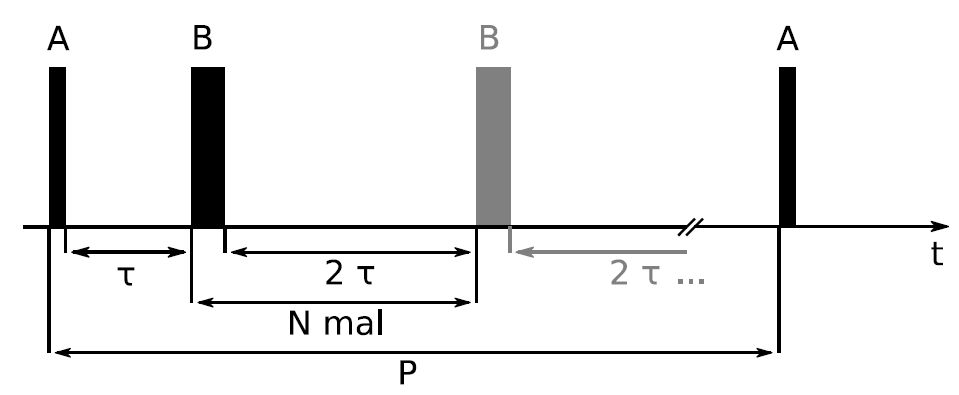
\includegraphics[width=0.8\textwidth]{images/pulsfolge.png}
    \caption{Einstellbare Parameter einer Pulsfolge \cite{V49}}
    \label{fig:pulsfolge}
\end{figure}

\subsection{Justierung}
\label{ssec:Justierung}

Vor der eigentlichen Messung muss die verwendete Apperatur justiert werden und bestimmte Parameter müssen abgestimmt werden.
Damit hier die Relaxationszeiten verkürzt werden wird statt einer Wasser-Probe
eine mit Kupersulfat ($\symup{CuSO}_4$) versetzte Wasser-Probe verwendet.

Es wird die Frequenz und Phase der Referenzsignale so eingestellt, 
dass die Messung des FID keine Schwingungen aufweist und hauptsächlich auf einem der beiden Signale zu sehen ist.
Dieses Signal wird dann als Realteil angesehen.

Der Feldgradient wird durch sogenanntes \enquote{shimmen} so eingestellt, dass der FID möglichst lang ist.

Zum Schluss der Justierung werden die Pulslängen so bestimmt, 
dass für den $\SI{90}{\degree}$-Puls die Amplitude der FID maximal wird
und für den $\SI{180}{\degree}$-Puls die Amplitude der FID minimal wird.

\subsection{Messung von \texorpdfstring{$T_1$}{T1}}
\label{ssec:T1_messung}

Die Pulslängen von $A$ und $B$ werden so eingestellt, dass zuerst ein $\SI{180}{\degree}$-Puls und dann ein $\SI{90}{\degree}$-Puls gesendet werden.
$N$ sollte 1 sein.
Nun ist $\tau$ logarithmisch zu variieren und die Amplitude der FID abzulesen.

\subsection{Messung von \texorpdfstring{$T_2$}{T2}}
\label{ssec:T2_messung}

Mit der Meiboom-Gill-Methode wird nun $T_2$ gemessen, also muss der Schalter MG auf on stehen.
Also sollte $A$ ein $\SI{90}{\degree}$-Puls und $B$ ein $\SI{180}{\degree}$-Puls sein.
Allerdings werden viele $B$-Pulse benötigt, also wird $N$ auf 100 gestellt.
Nun ist ein $\tau$ zu finden bei dem die FID Amplitude des letzten Pulses etwa $1/3$ der Amplitude des erste Pulses entspricht.
Der Output des Oszilloskops ist nun auf einem USB-Stick zu speichern.
Außerdem wird zum Vergleich der Output des Oszilloskops gespeichert wenn MG auf off steht.

\subsection{Diffusionsmessung}
\label{ssec:Diffusionsmessung}

Um die Diffusion gut messen zu können, wird nun nicht mehr der optimale $z$-Gradient benutzt sondern der maximale $z$-Gradient.
$A$ ist wieder ein $\SI{90}{\degree}$-Puls und $B$ ein $\SI{180}{\degree}$-Puls, allerdings diesmal mit $N=1$.

Nun wird bei verschiedenen Werten von $\tau$ die Amplitude des Echos gemessen bis das Echo im Rauschen verschwindet.

Das Echo, das am klarsten zu erkennen ist wird einzeln auf dem USB-Stick gespeichert und später für die Fouriertransformation verwendet.
